\documentclass[tikz]{standalone}
\usepackage{fontspec}
\renewcommand*{\familydefault}{\sfdefault}
\usepackage{standalone}
\usetikzlibrary{arrows.meta, decorations.pathreplacing, shapes.geometric}
\usetikzlibrary{bayesnet}

\begin{document}

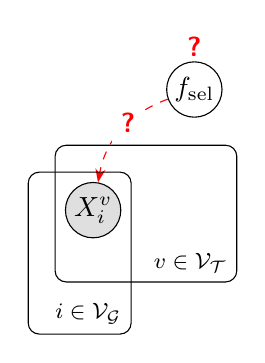
\begin{tikzpicture}

% Define nodes
\path (0,0)
node[obs] (X) {\(X^v_i\)}
to
(50:2.0 cm)
node[latent] (fsel) {\(f_\mathrm{sel}\)}
(X) +(1.7,0.7) coordinate (tree)
(X) +(-0.7,-1) coordinate (site)
;

\begin{scope}[font=\bfseries, pos=0.4, text=red]
\draw[dashed, red, -Stealth] (fsel) to[bend right] node[fill=white] {?} (X);
\path[anchor=south] (fsel) +(90:0.3 cm) node {?} ;
\end{scope}

% Plates
\plate {Xtree} {(X) (tree)} {\(v\in\mathcal{V}_\mathcal{T}\)} ;
\plate {Xsite} {(X) (site)} {\(i\in\mathcal{V}_\mathcal{G}\)} ;

\end{tikzpicture}

\end{document}
